\documentclass[12pt]{article}
\usepackage[utf8]{inputenc}
\usepackage[russian]{babel}
\usepackage{amssymb,amsmath}
\usepackage{amsmath}
\usepackage{amsthm}
\usepackage{hyperref}
\hypersetup{
    colorlinks,
    citecolor=black,
    filecolor=black,
    linkcolor=black,
    urlcolor=black
}
% \usepackage{biblatex}
\usepackage{graphicx}
\usepackage{parskip}
% \addbibresource{bibliography.bib}
\newtheorem{theorem}{Теорема}
\newenvironment{rowequmat}[1]{\left(\array{@{}#1@{}}}{\endarray\right)}
\textheight=24cm
\textwidth=16cm
\oddsidemargin=0pt
\topmargin=-1.5cm
\parindent=2cm
\title{Курсовой проект}
\author{\copyright Андрей Румянцев}
\date{29 ноября 2016}
\begin{document}
\begin{titlepage}
    \linespread{1.1}
    \begin{center}
    \fontsize{15pt}{15pt}\selectfont
    МИНЕСТЕРСТВО ОБРАЗОВАНИЯ РЕСПУБЛИКИ БЕЛАРУСЬ\\
    \vspace{0.5cm}
    БЕЛОРУССКИЙ ГОСУДАРСТВЕННЫЙ УНИВЕРСИТЕТ\\
    \vspace{0.5cm}
    \textit{ФАКУЛЬТЕТ ПРИКЛАДНОЙ МАТЕМАТИКИ И ИНФОРМАТИКИ}\\
    \vspace{0.5cm}
    \textit{КАФЕДРА МАТЕМАТИЧЕСКОГО МОДЕЛИРОВАНИЯ И АНАЛИЗА ДАННЫХ}\\
    \vspace{3.5cm}
    \fontsize{18pt}{18pt}\selectfont
    Румянцев\\
    Андрей Кириллович\\
    \vspace{0.5cm}
    \textbf{"Робастные оценки параметров регрессии при наличии группирования выборки"}\\
    \vspace{0.5cm}
    \fontsize{16pt}{16pt}\selectfont
    Курсовая работа\\
    \end{center}
    \vspace{3.5cm}
    \fontsize{14pt}{14pt}\selectfont
    \hspace{-0.25cm}
    \def\arraystretch{1.2}
    \begin{tabular}{l@{\hspace{3.25cm}}l}
    Допущен к защите & Научный руководитель:\\
    <<\underline{~~~~}>>~~\underline{~~~~~~~~~~~~} 2017 г&Агеева Елена Сергеевна\\
    Агеева Елена Сергеевна
    
    \end{tabular}
    \vspace{3cm}
    \begin{center}
    \fontsize{16pt}{16pt}\selectfont
    Минск, 2017
    \end{center}
  \end{titlepage}
\newpage
\tableofcontents
\newpage
\section{Введение}
Существует несколько подходов для оценки параметров регрессии, но далеко не все устойчивы к возникновениям аномальных наблюдений.
В реальной жизни аномальные наблюдения возникают постоянно, поэтому большинство методов просто неприменимо.
В прошлом веке в работах Хьюбера была заложена теория робастного оценивания.\hfill\break
Были предложены следующие робастные оценки\cite{Huber}:\hfill\break
\begin{itemize}
    \item М-Оценки\\
    \item R-Оценки\\
    \item L-Оценки
\end{itemize}
М-оценки -- некоторое подобие оценок максимального правдоподобия(ММП-оценки - частный случай), L-оценки строятся на основе линейных комбинаций порядковых статистик, R-оценки -- на основе ранговых статистик.
В данном курсовом проекте я буду моделировать функцию регрессии с аномальными наблюдениями, анализировать точность методов и находить для разных методов так называемый ''breakdown point''--процент аномальных наблюдений, при котором увеличение количества наблюдений не повысит точность методов.

\newpage
\section{Модель функции регрессии с аномальными наблюдениями и оценки ее параметров}
Введем линейную регрессию:\hfill\break
\begin{eqnarray}
    y_i=\beta_0+\beta_1 x_{i1}+\beta_2 x_{i2}+\dots+\beta_n x_{in}+\epsilon_i, i=\overline{1,N}\\
    \nonumber y_i= f(x_i,\beta)+\epsilon_i,\\
    \nonumber f(x_i,\beta)=\beta_0+\beta_1 x_{i1}+\beta_2 x_{i2}+\dots+\beta_n x_{in}
\end{eqnarray}
Или, в векторной форме:
\begin{equation}
    y_i= 
    \begin{pmatrix}
        \beta_0\\
        \beta_1\\
        \dots\\
        \beta_n
    \end{pmatrix}\times
    \begin{pmatrix}
        1\\
        x_{i1}\\
        \dots\\
        x_{in}
    \end{pmatrix}^{T}+ \epsilon_i,
\end{equation}
где $y_i$ -- $i$-е наблюдение из $N$ наблюдений($N$-объем выборки), $x_i=(x_{i1},x_{i2},\dots,x_{in})$ регрессоры, \{$\beta_k, k=\overline{0,n}$\}-- параметры регрессии, а $\epsilon_i$ -- случайная ошибка $i$-го эксперемента, распределение которой подчиняется нормальному закону с нулевым ожиданием и дисперсией $\sigma^2$.\hfill\break
В нашей задаче считаем параметры \{$\beta_k, k=\overline{0,n}$\} неизвестными, их нам и требуется найти.\hfill\break
Но мы будем рассматривать не линейную регрессию, заданную формулами (1)-(2), а линейную регрессию с аномальными наблюдениями вида:
\begin{equation}
    y_i^{\widetilde{\epsilon}}=(\xi_i)y_i+ (1-\xi_i)\eta_i,
\end{equation}
где $\xi_i$ принимает значение, равное 1, с вероятностью $1-\widetilde{\epsilon}$ и значение, равное 0, с вероятностью $\widetilde{\epsilon}$, т.е.:
\begin{equation}
    \begin{cases}
        p(\xi_i=0)=\widetilde{\epsilon}\\
        p(\xi_i=1)=1-\widetilde{\epsilon}
    \end{cases},
\end{equation}
которая называется функцией линейной регрессии с выбросами. $\eta_i$-случайная величина из какого-то другого неизвестного нам распределения. Переменную $\widetilde{\epsilon}$ будем называть процентом аномальных наблюдений.\hfill\break
Теперь рассмотрим некоторые методы оценки параметров регрессии:
\subsection{Метод Наименьших Квадратов}
Предлоположим, что случайные ошибки подчиняются нормальному закону распределения вероятностей:
\begin{equation}
    L\{\epsilon_i\}=N_1(0,\sigma^2), i = \overline{1,n}
\end{equation}
Строим логарифмическую функцию правдоподобия. В силу (1) и (2) имеем:
\begin{equation}
    L\{y_i\}=N_1(f(x_i;\beta), \sigma^2)
\end{equation}
Логарифмическая функция правдоподобия выглядит так\cite{Kharin}:
\begin{eqnarray}
    l(\beta)=\ln \prod_{i=1}^{n}(\frac{1}{\sqrt{2\pi}\sigma}e^{-\frac{(y_i-f(x_i;\beta))^2}{2\sigma^2}})=-\frac{1}{2}n\ln{2\pi\sigma^2}-\frac{1}{2\sigma^2}R^2(\beta),\\
    R^2(\beta)=\sum_{i=1}^{n}(\delta y_i)^2=\sum_{i=1}^{n}(y_i-f(x_i,\beta))^2\geq 0
\end{eqnarray}
Тогда оценка максимального правдоподобия из формул (4)-(5) такова:
\begin{eqnarray}
    \hat{\beta}=arg \min_{\beta}R^2(\beta)
\end{eqnarray}

\subsection{М-оценки}
Швейцарский статистик П.Хьюбер преложил использовать М-оценки \cite{Kharin}, которые являются решениями экстремальных задач вида:
\begin{eqnarray}
    \sum_{i=1}^{n}\phi(x_t;\beta)\rightarrow \min_{\beta},
\end{eqnarray}
где $\phi(\cdot;\beta)$-некоторая функция, определяющая конкретный тип оценок и их точность.\hfill\break
Очевидно, что $\phi(\cdot;\beta)\equiv - \ln{p(\cdot;\beta)}$-обычная оценка максимального правдоподобия, построенная по модели без выбросов (1).\hfill\break
Рассмотрим теперь некоторые способы выбора $\phi(\cdot;\beta)$.\hfill\break
\subsubsection{Способы выбора  функции для решения экстремальной задачи в M-оценках}
Для начала определим:
\begin{eqnarray}
    u_i=y_i^{\widetilde{\epsilon}}-(\beta_0+\beta_1 x_{i1}+\beta_2 x_{i2}+\dots+\beta_n x_{in})
\end{eqnarray}
Тогда существует такие методы\cite{RobustRegression}:\hfill\break
\begin{center}
\begin{tabular}{ |p{3cm}|p{10cm} | }
    \hline
    \multicolumn{2}{|c|}{Способы выбора $\phi(\cdot;\beta)$} \\
    \hline
    Метод& Целевая функция\\
    \hline
    Метод Наименьших Квадратов&$\phi(\cdot;\beta)_{OLS}=u^2$\\
    Хьюбера&$\phi(\cdot;\beta)_{H}=
        \begin{cases}
            \frac{1}{2}u^2, |u|\leq k,\\
            k|u|-\frac{1}{2}k^2, |u|>k
        \end{cases}$\\
    Биквадратный& $\phi(\cdot;\beta)_{B}=
    \begin{cases}
        \frac{k^2}{6}(1-[1-(\frac{u}{k})^2]^3), |u|\leq k\\
        \frac{k^2}{6}, |u|>k
    \end{cases}$\\
    \hline
\end{tabular}
\end{center}
\newpage
\section{Моделирование функции регрессии с аномальными наблюдениями}
Для начала смоделируем функцию регрессии по методу (3). Для удобства моделируем регрессию с одномерными регрессорами $x_i, i=\overline{1,N}$.\hfill\break
Воспользуемся такими параметрами:\hfill\break
\begin{center}
\begin{tabular}{|p{5cm}|p{5cm}|}
    \hline
    \multicolumn{2}{|c|}{Параметры программы} \\
    \hline
    Переменная&значение\\
    \hline
    Размер выборки $N$& 1000\\
    \hline
    Процент выбросов $\widetilde{\epsilon}$& 10\\
    \hline
    Параметры регрессии $\beta$& $(100,4)$\\
    \hline
    Регрессоры $x_i$ & $\sim U(-5,5)$\\
    \hline
    $\epsilon_i$&$\sim N(0,16)$\\
    \hline
    $\eta_i$&$\sim N(100,100)$\\
    \hline
\end{tabular},
\end{center}
$U(-5,5)$ - равномерное распределение на отрезке $[-5,5]$.\hfill\break
Получаем такой график:\hfill\break
\begin{figure}[ht!]
    \centering
    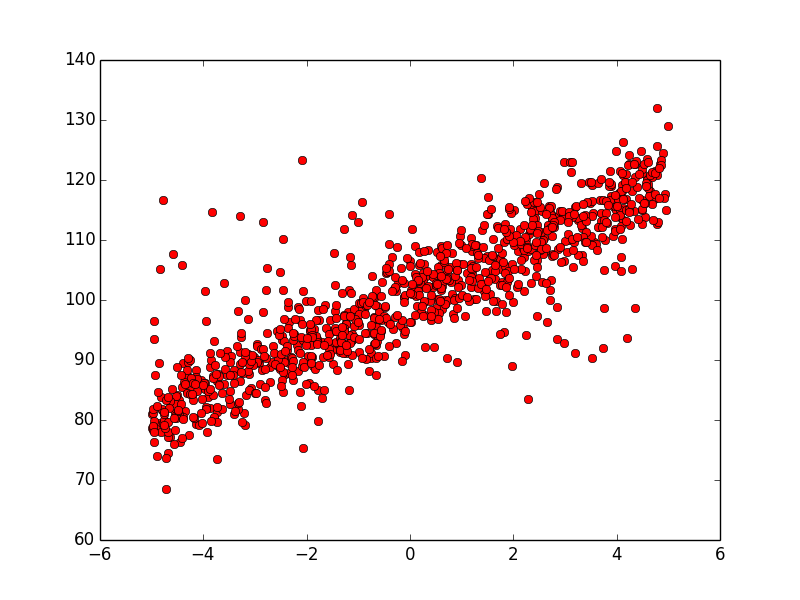
\includegraphics[width=100mm]{graphic.png}
    \caption{Вывод графика рассеяния $(y_i,x_i)$\label{overflow}}
\end{figure}
\newpage
\section{Поиск breakdown point у МНК и М-оценок}
Будем пользоваться той же моделью, как и в пункте 3.
Для поиска того процента загрязнений, при котором увеличение количества элементов выборки не повышает точности метода будем делать так:\hfill\break
\begin{itemize}
    \item Организуем цикл по процентам загрязнений $\widetilde{\epsilon}_i$ от $\widetilde{\epsilon}_0=0$ до $\widetilde{\epsilon}_{100}=100$, увеличивая каждый раз $\widetilde{\epsilon}_i$ на 1\\
    \item На каждой итерации будем 20 раз моделировать выборку с $N_1=1000$ и $N_2=3000$ наблюдений.
    На каждой такой итерации суммируем невязку с точными значениями параметров для каждого количества элементов, а потом находим среднее, поделив на количество суммирования, т.е. посчитаем усредненную невязку:
    \begin{eqnarray}
        \widetilde{\delta_1^{\widetilde{\epsilon}_i}}= \frac{1}{20}\sum_{k=1}^{20}(\sum_{i=0}^{n}(\beta_i-\hat{\beta_{N_1ki}})^2)^{\frac{1}{2}}\\
        \widetilde{\delta_2^{\widetilde{\epsilon}_i}}= \frac{1}{20}\sum_{k=1}^{20}(\sum_{i=0}^{n}(\beta_i-\hat{\beta_{N_2ki}})^2)^{\frac{1}{2}}
    \end{eqnarray}\\
    \item если полученная усредненная невязка при 1000 наблюдений меньше либо равна невязке при 3000 наблюдений, то заканчиваем цикл - нашли breakdown point, т.е.:
            \begin{eqnarray}
                br=
                \begin{cases}
                    \widetilde{\epsilon_i}, \textup{если}~ \widetilde{\delta_1^{\widetilde{\epsilon}_i}}<\widetilde{\delta_2^{\widetilde{\epsilon}_i}}
                \end{cases}
            \end{eqnarray}\\
    \item иначе повышаем процент на 1 и повторяем цикл: ~$\widetilde{\epsilon_{i+1}}=\widetilde{\epsilon_{i}}+1$
\end{itemize}
Такие тесты проведем для МНК и М-оценок.\hfill\break
\subsection{Результаты программы}
\begin{center}
\begin{tabular}{|p{8cm}|p{3cm}|}
    \hline
    \multicolumn{2}{|c|}{Найденные breakdown point для МНК и М-оценок} \\
    \hline
    Метод&breakpoint\\
    \hline
    МНК & 10\%\\
    М-оценка с функцией Хьюбера& 17\%\\
    \hline
\end{tabular}
\end{center}
Итак, видим, что М-оценки  значительно устойчивее к выбросам чем МНК.\hfill\break 
\newpage
\begin{figure}[ht!]
    \centering
    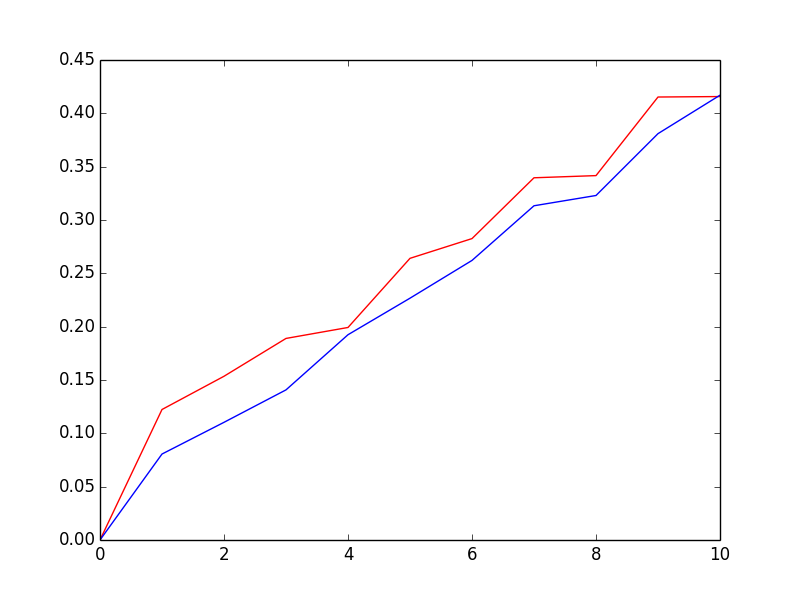
\includegraphics[width=100mm]{disperancies_MNK.png}
    \caption{График, на котором изображены $\widetilde{\delta_1^{\widetilde{\epsilon}_i}}~\textup{красным и}~\widetilde{\delta_2^{\widetilde{\epsilon}_i}}\textup{синим}$ относительно $\widetilde{\epsilon_i}$\label{overflow} в случае МНК}
\end{figure}
\begin{figure}[ht!]
    \centering
    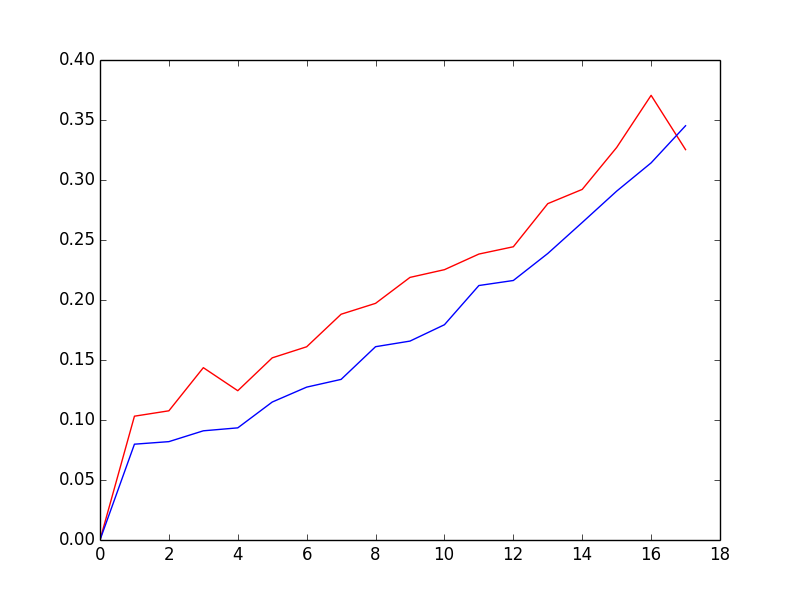
\includegraphics[width=100mm]{disperanciesMestimators.png}
    \caption{График, на котором изображены $\widetilde{\delta_1^{\widetilde{\epsilon}_i}}~\textup{красным и}~\widetilde{\delta_2^{\widetilde{\epsilon}_i}}\textup{синим}$ относительно $\widetilde{\epsilon_i}$\label{overflow} в случае М-оценок}
\end{figure}
 \hfill\break
\textbf{Замечания}:
\begin{itemize}
    \item Мы могли бы моделировать не 20 раз , а значительно больше, тем самым мы уменьшаем зависимость результата работы метода он моделируемой выборки.\\
    \item Аналогично можно заключить и для размера выборок(отношение моделируемых количеств можно значительно увеличить)
\end{itemize}
\newpage
\section{Построение оценки параметров регресии с помощью группирования выборки}
Будем работать с моделью регрессии (3), предполагая что имеем регрессию без выбросов (1). 
Каждый $y_i$ принадлежит нормальному распределению:
\begin{eqnarray}
    y_i=f(x_i,\beta)+\varepsilon_i \sim \mathcal{N}(f(x_i,\beta),\sigma^2)
\end{eqnarray}
Будем строить оценки таким образом: разделим множество значений функции регресси, т.е множество $\mathcal{R}$ на $k$ полуинтервалов:
\begin{eqnarray}
    \mathcal{R}=(-\infty,a_1]U(a_1,a_2]U\dots U(a_{k-1},+\infty )
\end{eqnarray}
Обозначим полученные интервалы: $\nu_0,\dots,\nu_{k-1}$.

Тогда:
\begin{eqnarray}
    P\{y_i\in\nu_j\}=
    \begin{cases}
        \frac{1}{2}(\textup{erf}(\frac{a_{j+1}-f(x_i,\beta)}{\sqrt{2}\sigma^2})-\textup{erf}(\frac{a_{j}-f(x_i,\beta)}{\sqrt{2}\sigma^2})),~j=\overline{1,k-2}\\
        \frac{1}{2}(1+\textup{erf}(\frac{a_{1}-f(x_i,\beta)}{\sqrt{2}\sigma^2})),~j=0\\
        \frac{1}{2}(1+\textup{erf}(\frac{a_{k-1}-f(x_i,\beta)}{\sqrt{2}\sigma^2})),~j=k-1
    \end{cases}
\end{eqnarray}, где
\begin{eqnarray}
    \textup{erf}(x)=\frac{2}{\sqrt{\pi}}\int_0^{x}e^{-t^2}
\end{eqnarray}
Все наблюдения $y_i$ отнесем к классам $\{\nu_i\}_{i=0}^{k-1}$ с помощью метода $k$-средних.
Тогда для каждого $y_i$ будем иметь класс $\mu_i$.
\begin{eqnarray}
    \mu_i=j, \textup{если $y_i$ отнесли к полуинтервалу $\nu_j$}
\end{eqnarray}
Понятно, что:
\begin{eqnarray}
    P(\mu_i=j|y_i\in \nu_j)=P(y_i\in \nu_{\mu_i})
\end{eqnarray}
Составим функцию правдоподобия:
\begin{eqnarray}
    L(\beta,\sigma^2, \nu_0,\dots, \nu_{k-1})=\textup{ln}(\prod_{i=1}^{n}P(\mu_i=j|y_i\in \nu_j))=\\
    =\sum_{i=1}^{n}\ln(P(\mu_i=j|y_i\in \nu_j))
\end{eqnarray}
Известно приближение для функции $\textup{erf}(x)$:
\begin{eqnarray}
    (\textup{erf} x)^2\approx 1- \exp(-x^2 \frac{\frac{4}{\pi}+ax^2}{1+ax^2}),\\
    a=\frac{8}{3\pi}\frac{3-\pi}{\pi -4}
\end{eqnarray}
Оно считается достаточно точным для $x$ близких к $0$ и к $\infty$ \cite{Winitzki}. \hfill\break
Найдем сразу производную для этого приближения:
\begin{eqnarray}
    \textup{erf}'(x) = \exp(-x^2 \frac{\frac{4}{\pi}+ax^2}{1+ax^2}) \frac{-2x\frac{\frac{4}{\pi}+ax^2}{1+ax^2}+(2ax^3)\frac{\frac{4}{\pi}+ax^2}{1+ax^2}-\frac{2ax^3}{1+ax^2}}{2\sqrt{1- \exp(-x^2 \frac{\frac{4}{\pi}+ax^2}{1+ax^2})}}
\end{eqnarray}
Будем максимизировать функцию $L$.
Для этого будем искать нули ее производной с помощью вычислительных методов(например, метод Ньютона).
\begin{eqnarray}
    \frac{\delta L}{\delta \beta}=\frac{\delta \sum_{i=1}^{n}\ln(P(\mu_i=j|y_i\in \nu_j))}{\delta \beta}=\frac{\delta \sum_{i=1}^{n}\ln P(y_i\in \nu_{\mu_i})}{\delta \beta}=\\
    =\frac{\delta \sum_{i=1}^{n} \ln(\frac{1}{2}(\textup{erf}(\frac{a_{\mu_i+1}-f(x_i,\beta)}{\sqrt{2}\sigma^2})-\textup{erf}(\frac{a_{\mu_i}-f(x_i,\beta)}{\sqrt{2}\sigma^2})) )         }{\delta \beta}=\\
    =  \sum_{i=1}^{n} \frac{(\textup{erf'}(\frac{a_{\mu_i+1}-f(x_i,\beta)}{\sqrt{2}\sigma^2})-\textup{erf'}(\frac{a_{\mu_i}-f(x_i,\beta)}{\sqrt{2}\sigma^2}))}{ (\textup{erf}(\frac{a_{\mu_i+1}-f(x_i,\beta)}{\sqrt{2}\sigma^2})-\textup{erf}(\frac{a_{\mu_i}-f(x_i,\beta)}{\sqrt{2}\sigma^2}))}  (-1) \frac{\delta f(x_i,\beta)}{\delta \beta} )=
\end{eqnarray}
% \section{Список литературы}
% \printbibliography
\begin{thebibliography}{9}
    \bibitem{Huber}
    Хьюбер Дж П.,
    \textit{Робастность в статистике:пер. с англ.}.
    М.:Мир,1984-304с

    \bibitem{Kharin}
    Харин Ю.С., Зуев Н.М.,
    Жук Е.Е,
    \textit{Теория вероятностей, математическая и прикладная статистика: учебник}
    Минск: БГУ, 2011.-463с

    \bibitem{RobustRegression}
    John Fox \& Sanford Weisberg,
    \textit{Robust Regression},
    October 8, 2013

    \bibitem{RobustPolynomialEstimation}
    А.В. Омельченко,
    \textit{Робастное оценивание параметров полиномиальной регрессии второго порядка,}
    Харьковский национальный университет радиоэлектроники, Украина, 2009

    \bibitem{ComparisonRobust}
    \"{O}zlem G\"{u}r\"{u}nl\"{u} Alma,
    \textit{Comparison of Robust Regression Methods
    in Linear Regression},
    Int. J. Contemp. Math. Sciences, Vol. 6, 2011, no. 9, 409 - 421

    \bibitem{ComparisonRobust}
    \"{O}zlem G\"{u}r\"{u}nl\"{u} Alma,
    \textit{Comparison of Robust Regression Methods
    in Linear Regression},
    Int. J. Contemp. Math. Sciences, Vol. 6, 2011, no. 9, 409 - 421

    \bibitem{Winitzki}
    Sergei Winitzki,
    \textit{A handy approximation for the error function and its inverse}
\end{thebibliography}
\addcontentsline{toc}{section}{Список Литературы}
\end{document}